\documentclass{article}
\usepackage{cmap}						% Улучшенный поиск русских слов в полученном pdf-файле
\usepackage[T2A]{fontenc}				% Поддержка русских букв
\usepackage{fontenc}				    % Поддержка русских букв
\usepackage{hyperref} 
\usepackage[utf8]{inputenc}				% Кодировка utf8
\usepackage[english, russian]{babel}	% Языки: русский, английский
\usepackage{amsthm,amsfonts,amsmath,amssymb,amscd} % Математические дополнения от AMS
\usepackage{graphicx} % Подключаем пакет работы с графикой

\usepackage{graphicx}  % Для вставки рисунков
\usepackage[update,prepend]{epstopdf} % EPS-рисунки конвертируются в PDF
\usepackage{wrapfig} % Обтекание рисунков текстом
\usepackage[usenames,dvipsnames,svgnames,table,rgb]{xcolor}
\usepackage{float}

 \usepackage{geometry} % Простой способ задавать поля
 \geometry{top=30mm}
 \geometry{bottom=25mm}
 \geometry{left=20mm}
 \geometry{right=15mm}

\newcolumntype{C}[1]{>{\centering\arraybackslash}m{#1}}
 

\begin{document}

\begin{titlepage}  

\begin{center}  

\large Национальный исследовательский университет \\"Высшая школа экономики"\\[0.5cm]

\large Факультет компьютерных наук\\

\large Департамент анализа данных и искусственного интеллекта\\[4cm]

\huge Домашнее задание\\
\large по анализу и разработке данных\\[4cm]

\end{center}

\begin{flushleft}
\large Выполнили студенты БПМИ133:\\
\large \bf{Стеценко Макар}\\
\large \bf{Корытова Александра}\\
\large \bf{Милеев Алексей}\\[5cm]
\end{flushleft}

\begin{center}
\large Москва 2015
\end{center}

\end{titlepage}

\newpage


\large \textbf{Домашнее задание №1}

1. В настоящих данных приводится статистика по NEA (Near Earth Objects) и кометам, обнаруженным иследовательской миссией NEOWISE под руководством NASA. Near-Earth Objects - это кометы и астероиды, которые были притянуты гравитационным полем ближайщих планет, в следствии чего они смогли сблизиться с Землей. \\[0.3cm]



Каждый объект описывается следующим набором признаков:

\begin{itemize}
\item {Discovery Date [Дата открытия]} 

Качественный признак в формате YYYY-MM-DD

\item {H (mag) [Магнитуда]}

Количественный признак, абсолютная величина

С помощью абсолютной магнитуды вычисляется диаметр астероида, чем ниже значение H, тем больше размер объекта.

\item {MOID (AU) - Minimum Orbit Distance [Минимальная дистанция орбиты]}

Количественный признак, измеряемый относительно AU (The astronomical unit).

//AU - астрономическая единица измерения длины, приближенно показывающая расстояние между Землей и Солнцем. Равна 149597870700 метров (примерно 150 млн км).

Minimum orbit intersection distance (MOID) - мера, используемая в астрономии для оценки потенциальных сближений и рисков столкновений между астрономическими объектами.

\item {q (AU) perihelion distance}

Количественный признак

Perihelion - точка на орбите планеты, кометы или другого объекта, расстояние от которой до Солнца минимально.

\item {Q (AU) aphelion distance}

Количественный признак

Aphelion - точка, в которой небесное тело максимально удалено от Солнца.

\item {period (yr) [Период]}

Количественный признак, показывающий период обращения объекта вокруг Солнца, измеряется в годах.


\item {PHA (Potentially Hazardous Asteroids)}

Признак, показывающий принадлежит ли астероид к классу PHA. 
Принимает два значения (Y/N), для удобства можно считать количественным. 

\item {Orbit Class [Класс орбиты]}

Качественный признак, множество принимаемых значений: \{Apollo, Aten, Amor, Atiras\}.\\[0.3cm]

\end{itemize} 

2. Предметная область\\[0.15cm]

Научный интерес к таким объектам проявлен во многом из-за их происхождения. Так, например, астероиды по сути являются уцелевшими осколками после формирования нашей солнечной системы. Поскольку эти объекты могут столкнуться, они оказывали и будут оказывать влияние на биосферу Земли. Так же астероиды являются богатым источником ресурсов. Выяснилось, что минеральных запасов в астероидном поисе Марса и Юпитера хватит, чтобы каждому человеку на Земле дать 100 миллиардов долларов.

По имеющимся данным можно пробовать строить модели для определения принадлежности небесного объекта к классу PHA. \\[1cm]

Источник: \href{http://neo.jpl.nasa.gov/stats/wise/}{http://neo.jpl.nasa.gov/stats/wise/}. 

\vspace{.2cm}
\large \textbf{Домашнее задание №2}
\vspace{.2cm}

1. Был выбран количественный признак H (mag) [Магнитуда]. Поскольку этот признак позволяет определить размер исследуемого объекта, то его подробное изучение позволит лучше понять, каких размеров достигают наиболее встречаемые астероиды. В используемом наборе данных H принимает следующие значения: \\[0.15cm]
 \noindent 15.6 16.2 17.0 17.5 18.3 18.3 18.7 18.7 18.9 19.0 19.1 19.2 19.2 19.3 19.3 19.3 19.4 19.4 19.4 19.5 19.5 19.5
 19.6 19.6 19.7 19.7 19.7 19.7 19.8 19.9 19.9 19.9 20.0 20.1 20.1 20.2 20.2 20.3 20.3 20.4 20.6 20.7 20.7 20.7
 20.7 20.8 20.8 20.8 20.9 20.9 20.9 21.0 21.0 21.1 21.3 21.4 21.4 21.5 21.5 21.6 21.8 21.8 22.0 22.1 22.3 22.5
 22.6 22.6 23.2 24.1 \\[0.15cm]
Построим гистрограму: 

\begin{figure}[H] 
\centering
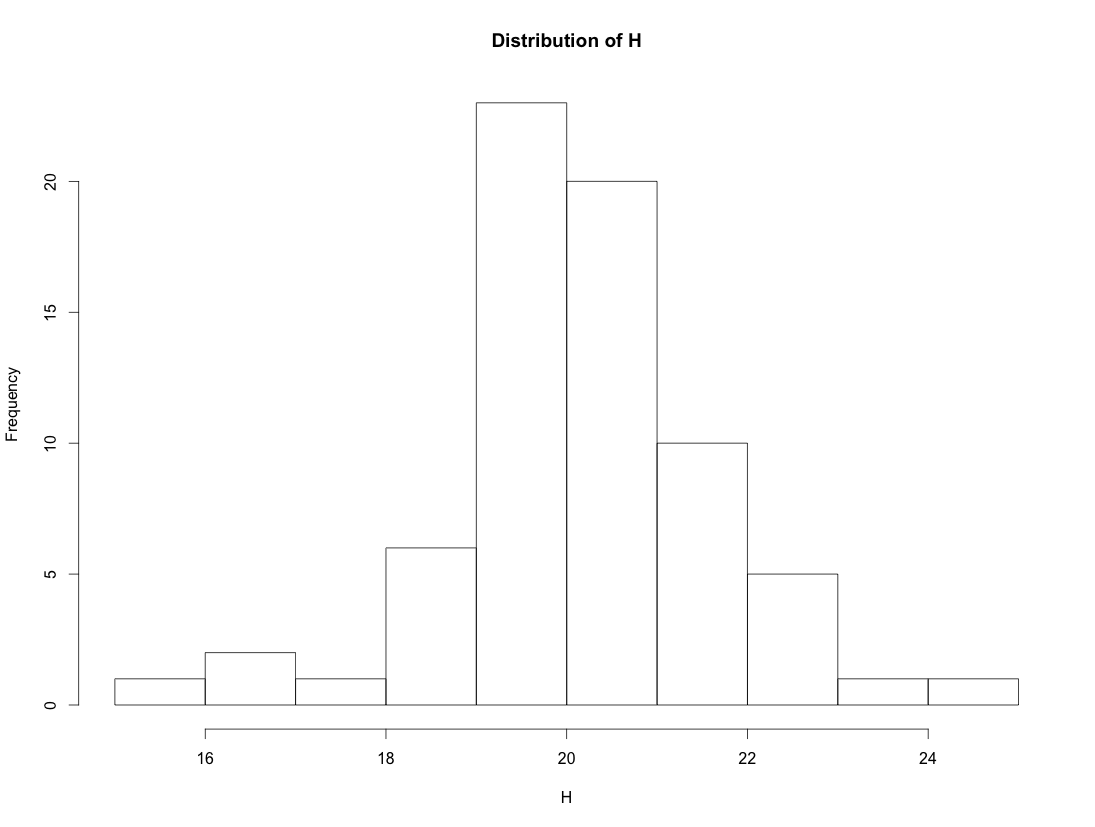
\includegraphics[scale=0.4]{img/2_hist.png}
\caption{Гистограмма для признака H (mag)}
\label{fig :metka1}
\end{figure}

Полученная гистограмма позволяет нам предположить, что распределение признака H похоже на нормальное. А также понять, в каком диапазоне лежат наиболее встречаемые значения H (примерно от 19 до 21). Этот факт подтвердится, когда мы найдем моду. Построим бокс-плот:

\begin{figure}[H] 
\centering
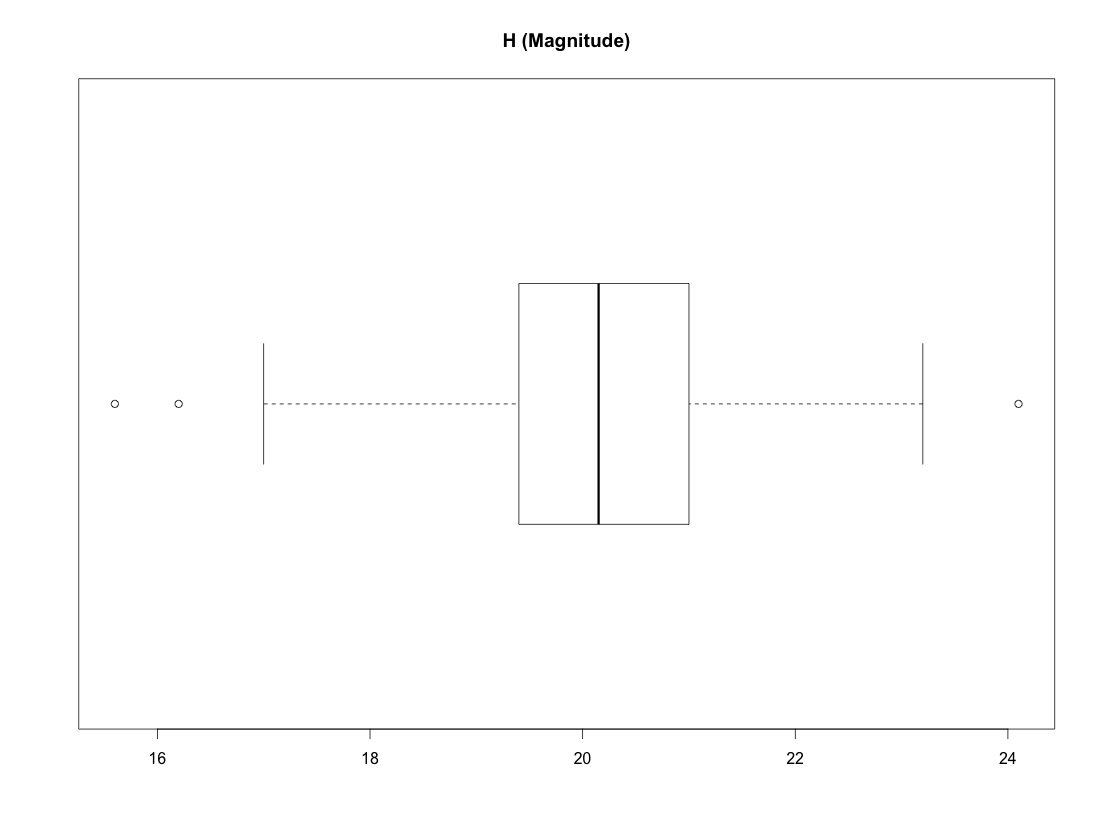
\includegraphics[scale=0.4]{img/2_box.png}
\caption{Бокс-плот для H (mag)}
\label{fig :metka2}
\end{figure}

Видно, что у нас есть 3 выброса, а именно: [16.2, 24.1, 15.6]. Так же видно значение медианы.

Найдем среднее значение, моду и медиану

\begin{center}
  \begin{tabular}{| C{2.5cm} | C{2.5cm} | C{2.5cm} | @{}m{0pt}@{}}
    \hline
    Среднее & Медиана & Мода &\\[0.5em] \hline
    20.21 & 20.15 & 19.7 и 20.7 &\\[0.5em]   
    \hline
  \end{tabular}
\end{center}

Как видно, найденные значения не равны, это свидетельствует о том, что величина H не подчиняется нормальному распределению, а немного отклоняется от него. Однако, если убрать из расчетов найденные выбросы [16.2, 24.1, 15.6] и пересчитать, то получим равные между собой значения:

\begin{center}
  \begin{tabular}{| C{2.5cm} | C{2.5cm} | C{4.5cm} | @{}m{0pt}@{}}
    \hline
    Среднее & Медиана & Мода &\\[0.5em] \hline
    20.2 & 20.2 & (19.7 + 20.7) / 2 = 20.2 &\\[0.5em]   
    \hline
  \end{tabular}
\end{center}

2. Теперь построим доверительные интервалы тремя методами:
\begin{enumerate}
    \item Статистический
    \item Опорный бутстрэп
    \item Безопорный бутстрэп
\end{enumerate}

Так как наше распределение похоже на нормальное, то
$$CI = \left(mean - 1.965 \frac{std}{\sqrt{n}}; mean + 1.965 \frac{std}{\sqrt{n}}\right)$$
$$CI = (19.859740; 20.560260)$$

Для 5000 средних значений от случайных выборок с повторениями построим гистограмму:

\begin{figure}[H] 
\centering
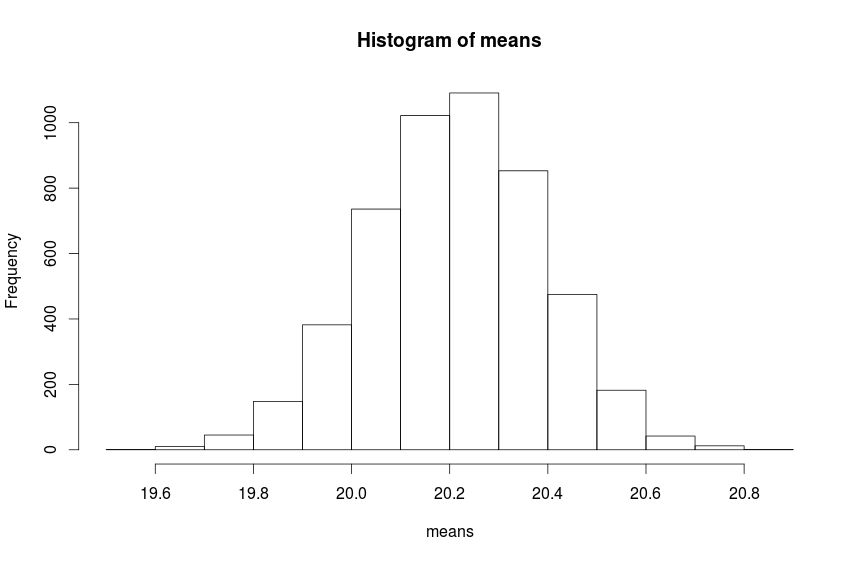
\includegraphics[scale=0.4]{img/2_pivotal.png}
\caption{Гистограмма для признака средних значений}
\label{fig :metka1}
\end{figure}

Видим, что гистограмма похожа на нормальное распределение, а значит применяем метод опорного бутстрэпа и получаем интервал:
$$PCI = (20.207460; 20.217272)$$

И теперь безопорный бутстрэп:
$$NPCI = (19.864286; 20.542857)$$

3. Покажем, что для моды и медианы нельзя использовать технику опорного бутстрэпа.

Для это построим гистограммы аналогично случаю со средним.

\begin{figure}[H] 
\centering
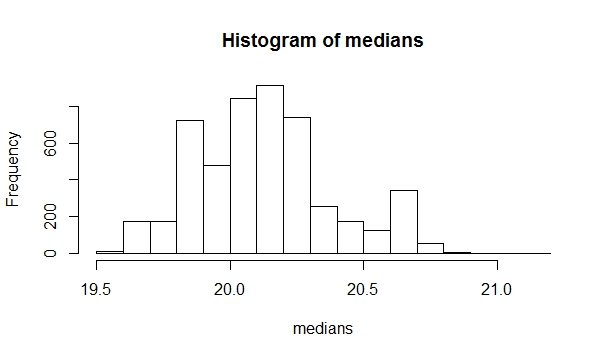
\includegraphics[scale=0.6]{img/2_medians.jpeg}
\caption{Гистограмма для медиан}
\label{fig :metka1}
\end{figure}


\begin{figure}[H] 
\centering
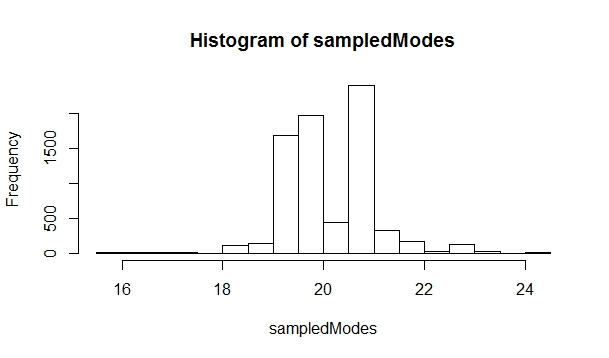
\includegraphics[scale=0.6]{img/2_modes.jpeg}
\caption{Гистограмма для мод}
\label{fig :metka1}
\end{figure}

Видим, что распределения совсем не напоминают Гауссовские. 

Значит, мы можем использовать только безопорный бутстрэп.

$$$$

Доверительный интервал для медианы:

$$NPCI = (19.700000; 20.700000)$$

$$$$

Доверительный интервал для моды:

$$NPCI = (18.300000; 20.700000)$$

$$$$

\large \textbf{Домашнее задание №3}

1. Построим диаграмму разброса для имеющихся признаков:

\begin{figure}[H] 
\centering
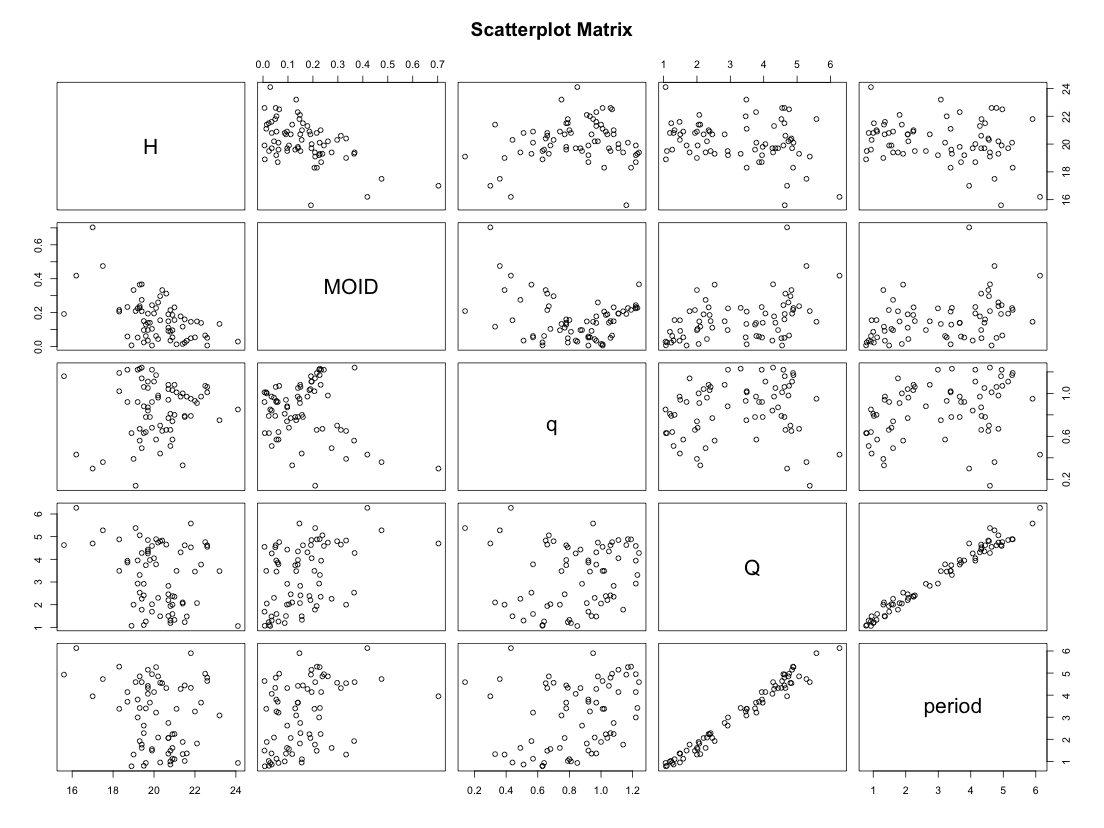
\includegraphics[scale=0.5]{img/3_paired_scatter.png}
\caption{Матрица разброса}
\label{fig :metka1}
\end{figure}

Пара Q и period больше всего напоминает линейную зависимость. Рассмотрим ee отдельно:  

\begin{figure}[H] 
\centering
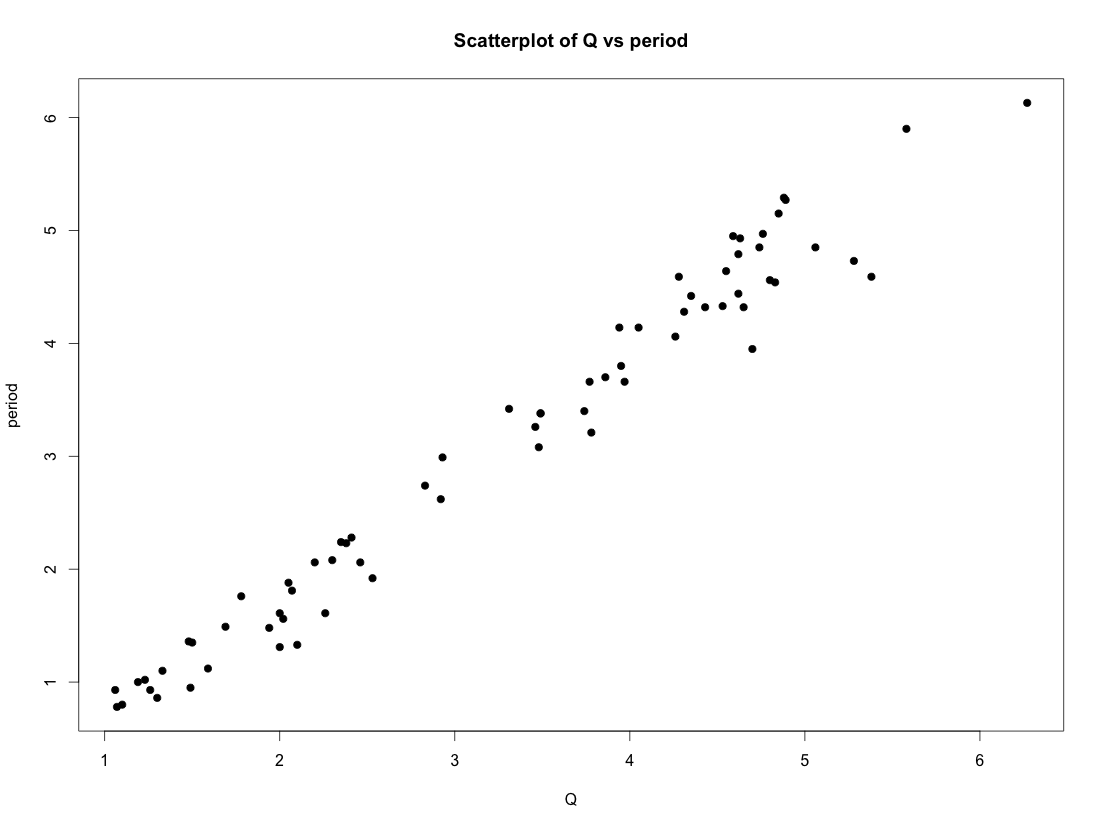
\includegraphics[scale=0.4]{img/3_Q_vs_period.png}
\caption{Диаграмма разброса Q и period}
\label{fig :metka1}
\end{figure}

Такую сильную зависимость можно объяснить тем, что Q - это точка, в которой небесное тело максимально удалено от Солнца, а period - это период обращения объекта вокруг Солнца. Чем дальше объект от солнца, тем больше его период. Поскольку, при обнаружении астероида, зная точку, в которой небесное тело максимально удалено от Солнца, можно высчитать период, то Q мы будем считать за Х, а период за Y.

2. Теперь найдем коэффициенты линейной регрессии $Y = aX+b$:

\begin{center}
  \begin{tabular}{| C{2.5cm} | C{2.5cm} | @{}m{0pt}@{}}
    \hline
    a & b &\\[0.5em] \hline
    1.075 & -0.424 &\\[0.5em]   
    \hline
  \end{tabular}
\end{center}

Построим график разброса с нанесенной моделью:

\begin{figure}[H] 
\centering
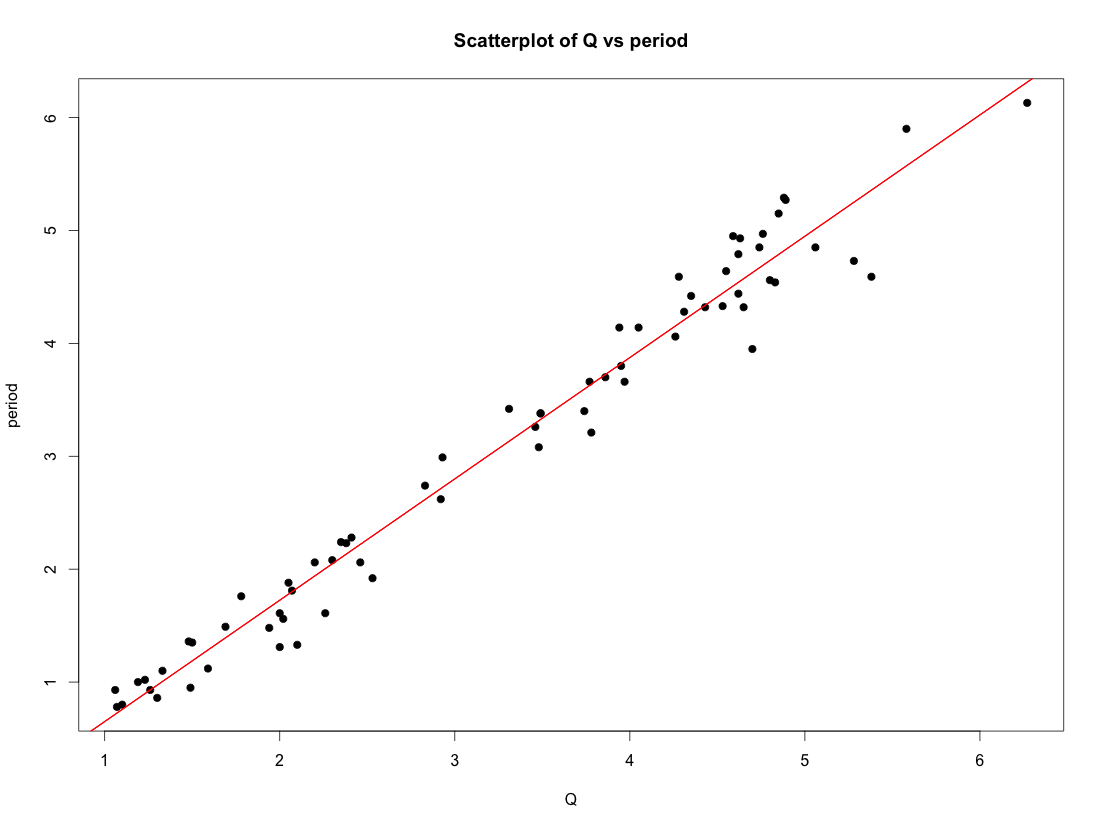
\includegraphics[scale=0.4]{img/3_regression.png}
\caption{Диаграмма разброса Q и period и линейная модель}
\label{fig :metka1}
\end{figure}

Коэффициент а обозначает на сколько изменится признак period, если увеличить Q на малую величину. В данном случае, при увеличении Q на единицу, period вырастет на 1.075.

\noindent 3. Найдем среднюю ошибку предсказания (Mean Absolute Error), она будет равна:
$$
MAE = \frac{1}{n} \sum_{k=1}^n |period_k - (aQ_k+b)|
$$

\begin{center}
  \begin{tabular}{| C{2.5cm} | @{}m{0pt}@{}}
    \hline
    MAE &\\[0.5em] \hline
    0.2095 &\\[0.5em]   
    \hline
  \end{tabular}
\end{center}

Данная величина говорит нам, что в среднем предсказанное моделью значение отличается от имеющихся в выборке данных на 0.21. Чем меньше данная ошибка, тем больше мы можем доверять построенной модели.

4. Коэффициент детерминации равен 0.97. Коэффициент детерминации объясняет долю дисперсии Y регрессией на X. Таким образом, мы получили, что наша модель объясняет 97\% дисперсии Y, это очень хороший показатель.

Корреляция признаков period и Q равна 0.984. Значение коэффициента корреляции указывает на то, как близко к прямой  находятся точки на диаграмме рассеивания, в частности, значение $\pm 1$ означает точное совпадение, а значение близкое к 0, говорит об отсуствии линейной корреляции. Знак + коэффициента означает, что значение period увеличивается с ростом Q. 

Коэффициент детерминации равен квадрату коэффициента корреляции.

Согласно полученным значениям коэффициентов, для нашей модели мы имеем положительную связь признаков. 

Безусловно, гипотеза о существовании линейной связи между признаками Q и period подтвердилась. Мы получили достаточно близкие к 1 значения коэффициентов корреляции и детерминации, это значит, что построенная регрессия довольно точно отражает реальное положение дел. 

\end{document}